\section{Experimental Results and Discussion}

%%%% BECHMARKS
\begin{table*}
\caption{Benchmark results vs. our best results}
\begin{center}
\begin{small}
\begin{tabular}{lll}
\hline
\textbf{Task} & \textbf{Benchmark} & \textbf{Us} \\ \hline
POS-Tagging & (Accuracy) 97.24 \cite{Toutanova:2003} & 0.9592 (skip-gram negsam+up) \\ 
Chunking & (F1) 0.9429 \cite{Sha:2003} & 0.9386 (Brown cluster v2000+)\\  
NER & (F1) 0.8931 \cite{Ando:2005} & 0.8686 (skip-gram negsam+noup)\\  
MWE & (F1) 0.6253 \cite{Schneider+:2014} & 0.6546 (cw+up)\\ 
\hline
\label{benchmark}
\end{tabular}
\end{small}
\end{center}
\end{table*}

%%%%%%%%%%%%%%%%%%%%%%%%%%%%
%%% HEATMAPS 
\begin{figure*}
\caption{Best results for each method for POS-Tagging, Chunking, NER and MWE identification. The x-axis correspond to the different word embeddings methods and the y-axis to the 10 training partitions at log scale. Green color stand for high performance, while red color stands for low performance. The methods are in chronological order; wherein the suffix \textit{up} stands for \textit{updated or fine-tuned features}, and \textit{noup} stands for \textit{no-updated} features.}
\centering
\begin{subfigure}{7cm}
	\centering
    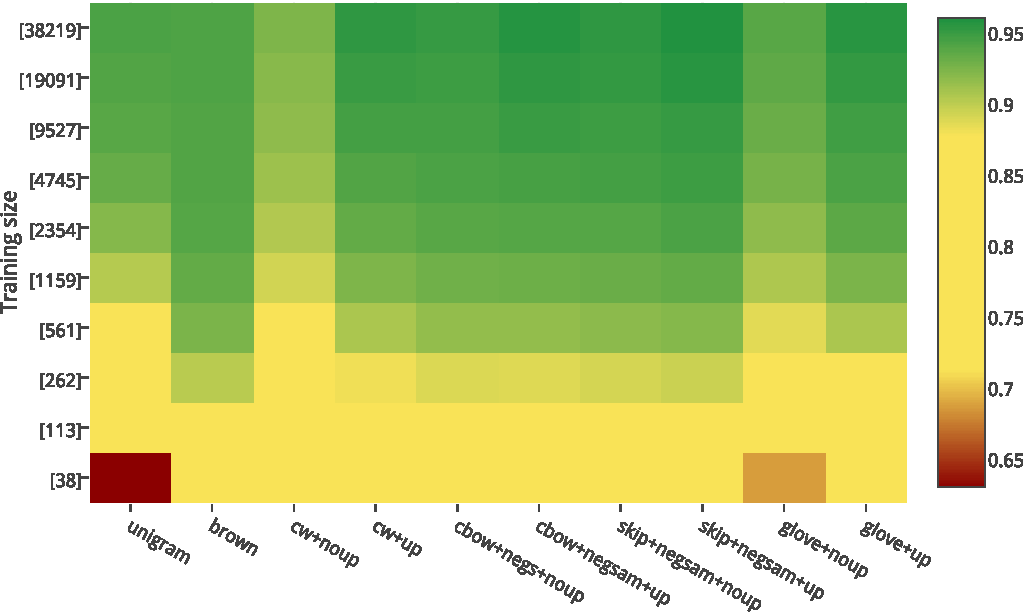
\includegraphics[scale=0.4]{plots/map-pos-color-invert}    	
	\subcaption{POS-Tagging Accuracy}	
	\label{pos}
\end{subfigure}
\begin{subfigure}{7cm}
	\centering
    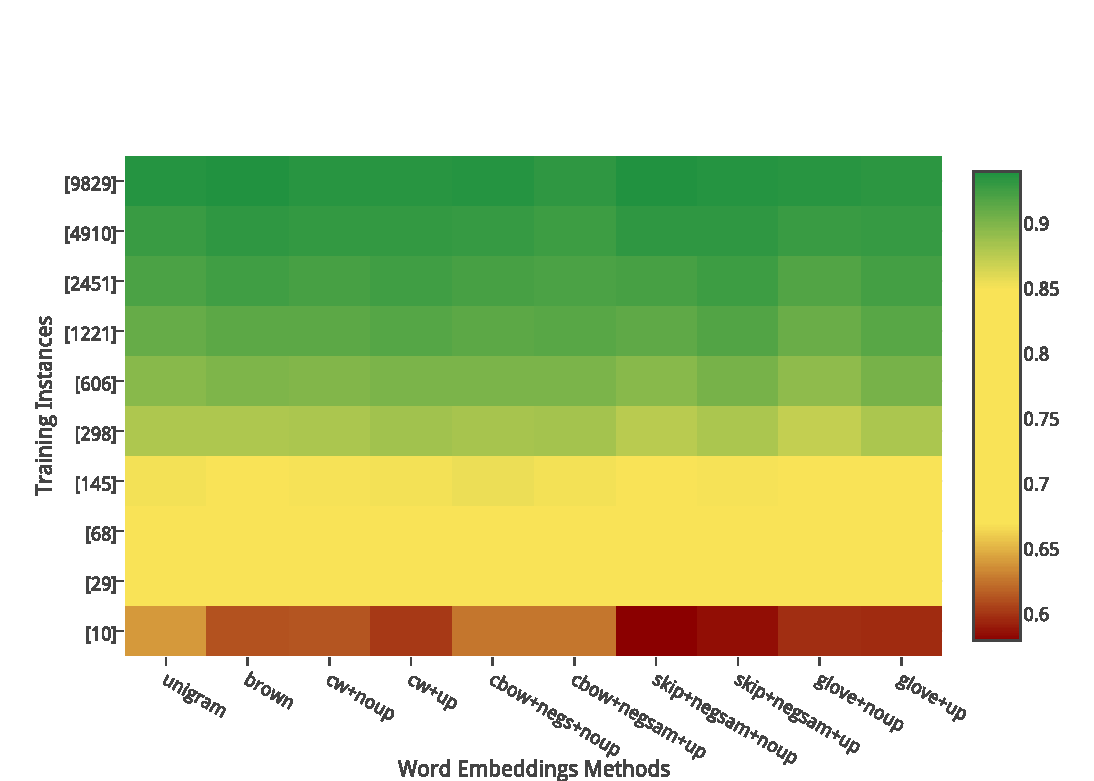
\includegraphics[scale=0.4]{plots/map-chunk-color-invert}
	\subcaption{Chunking F1-Measure}	
	\label{chu}
\end{subfigure}
%\\[-2ex]  %%<-- in this line
\begin{subfigure}{7cm}
	\centering
    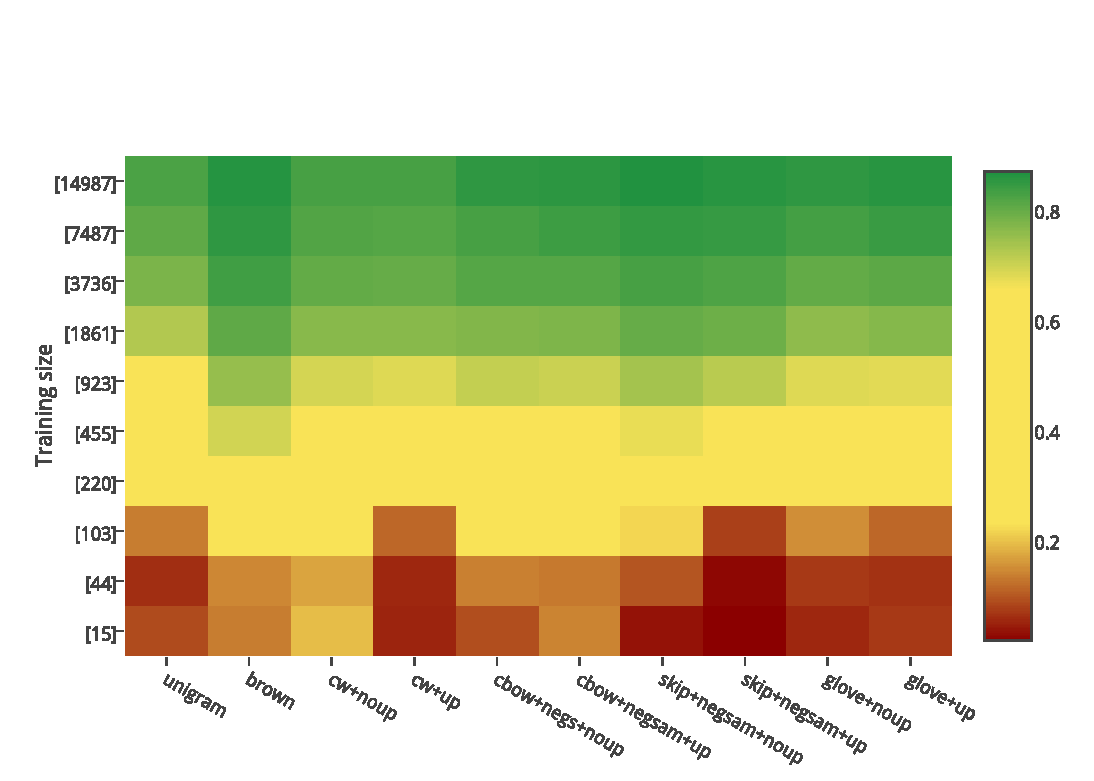
\includegraphics[scale=0.4]{plots/map-ner-color-invert}    	
	\subcaption{NER F1-Measure}	
	\label{ner}
\end{subfigure}
\begin{subfigure}{7cm}
	\centering
    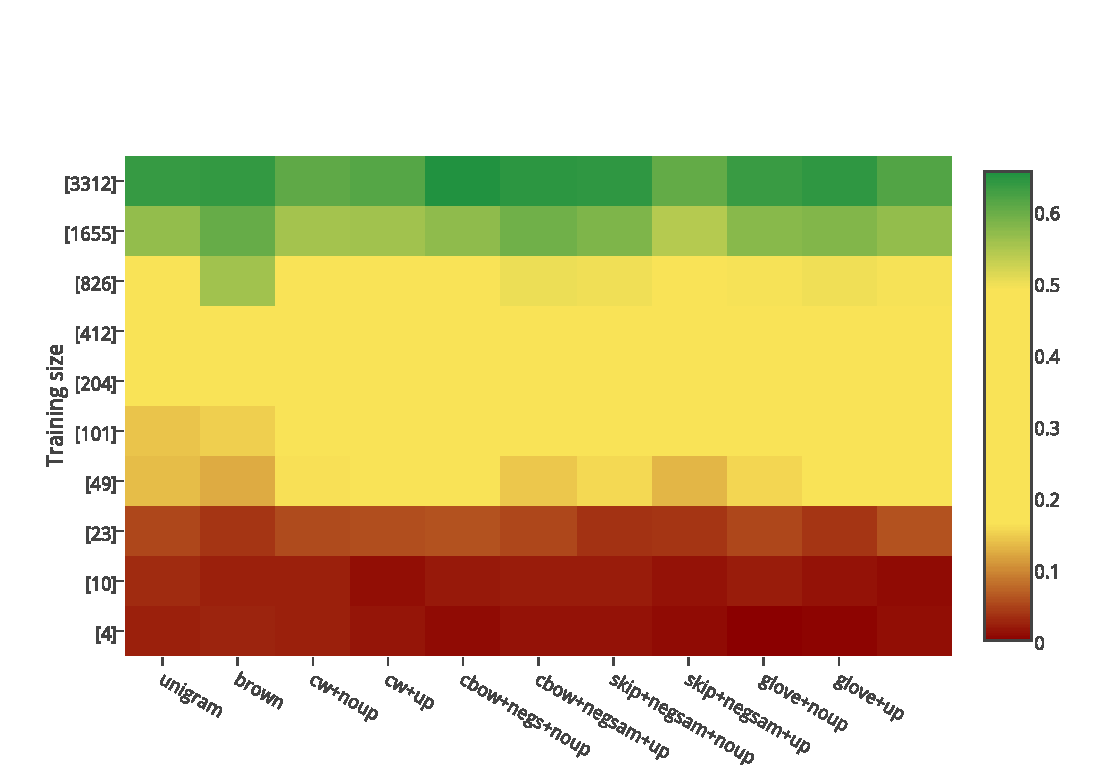
\includegraphics[scale=0.4]{plots/map-mwe-color-invert}
	\subcaption{MWEs F1-Measure}		
	\label{mwe}
\end{subfigure}
\label{fig:heatmaps}
\end{figure*}


%%%%%%%%%%%%%%%%%%%%%%%%%%%%
%%% Vector fields
% POS
\begin{figure*}
\caption{Updated vs. no-updated word representations for POS-tagging and chunking using skip-gram}
\centering
\begin{subfigure}[b]{0.48\textwidth}
	\centering
    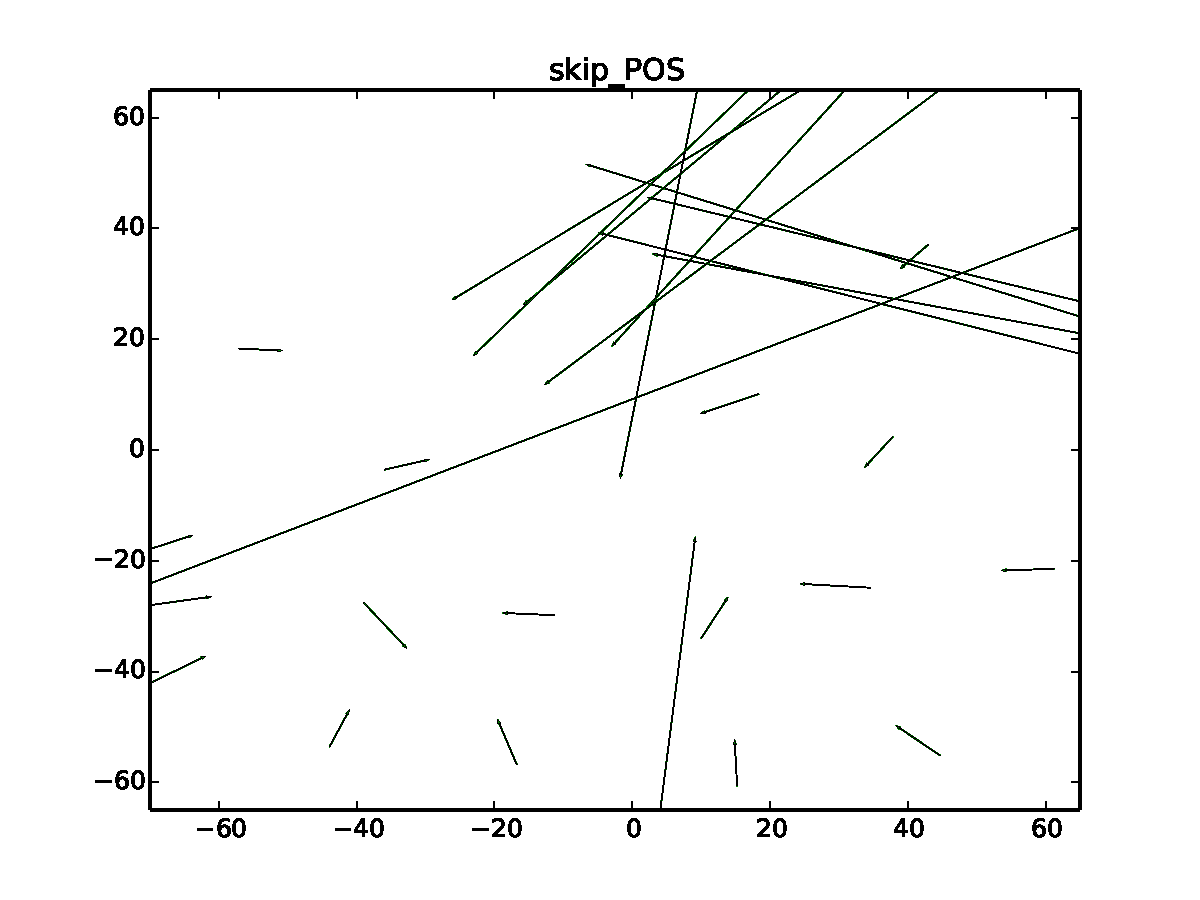
\includegraphics[width=\textwidth]{plots/vectorField/Lizhen/scaled/skip_POS}    	
	\label{fig:skippos}
	\subcaption{POS-tagging}	
\end{subfigure}
\begin{subfigure}[b]{0.48\textwidth}
	\centering
    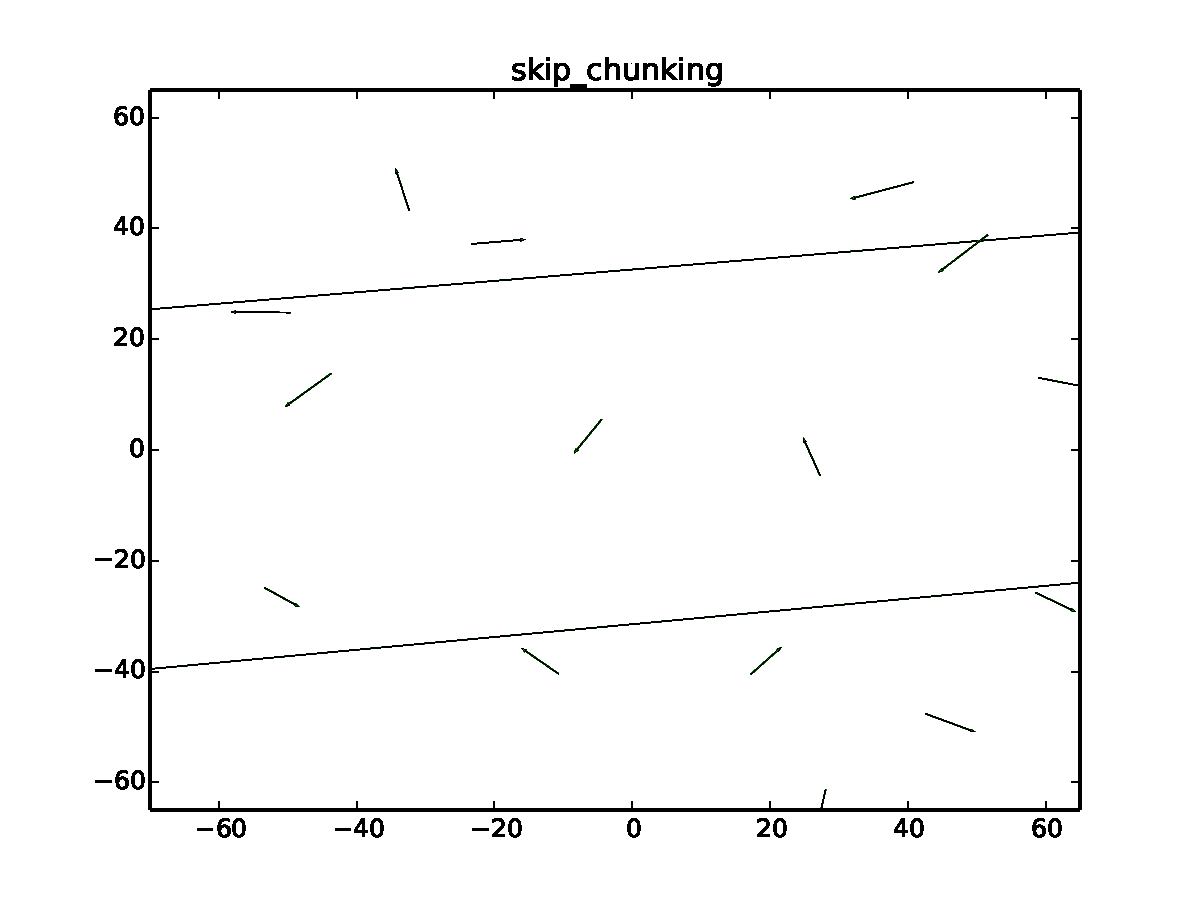
\includegraphics[width=\textwidth]{plots/vectorField/Lizhen/scaled/skip_chunking}
	\label{fig:skipChu}
	\subcaption{Chunking}	
\end{subfigure}
%\begin{subfigure}[b]{0.48\textwidth}
%	\centering
%   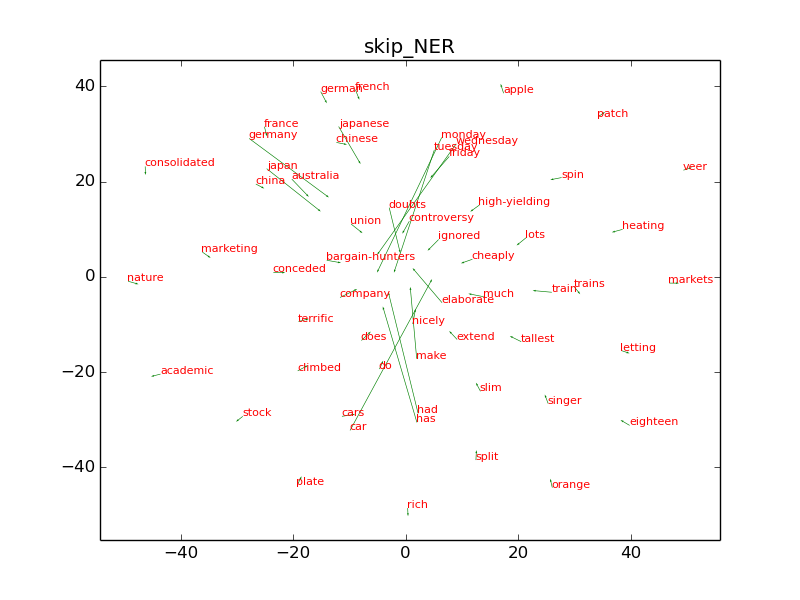
\includegraphics[width=\textwidth]{plots/vectorField/skip_NER.png}
%	\label{fig:skipner}
%	\subcaption{}	
%\end{subfigure}
%%\begin{subfigure}{6cm}
%	\centering
 %   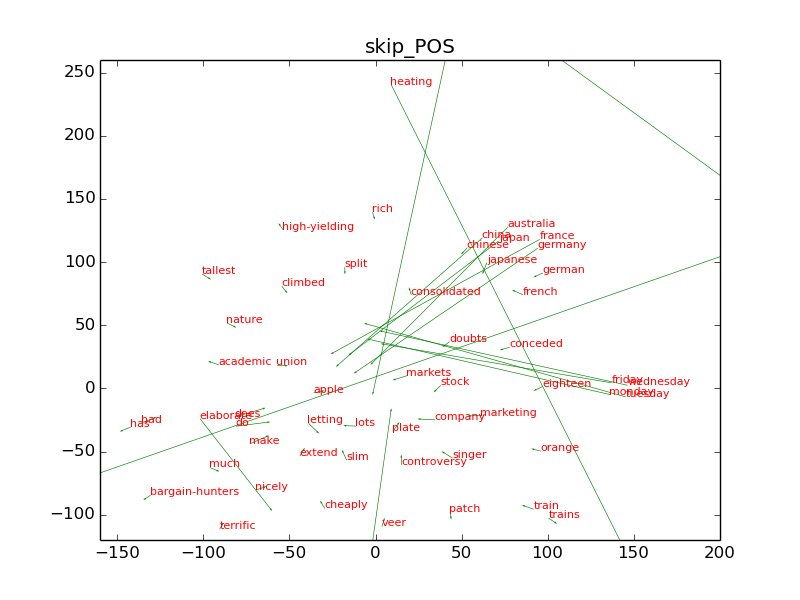
\includegraphics[scale=0.3]{plots/vectorField/skip_POS.png}
%	\label{fig:skipmwe}
%	\subcaption{}	
%\end{subfigure}
\label{fig:vectorfield}
\end{figure*}

We focus on the following questions:

\textbf{(i) Are the evaluated word embedding methods better than unigram features?}
To answer this question, we systematically compared the usefulness of word embedding versus
unigram features for sequence tagging and noted that word embedding methods always outperform 
unigram features (Figures \ref{fig:heatmaps}). 

\textbf{(ii) How does the size of labelled training data affect the experimental results?}
We observed that embedding methods are especially helping POS-tagging and NER when there are only several hundreds of training instances. 
Therefore, confirming that any of the evaluated word embedding methods should be used when POS-tagging or NER labelled data is limited.
These early improvements are less evident for chunking and MWE, and according to our results, all the methods, including unigram, needed the similar amount of training data to reach a decent performance.
%We attribute this to: a) the standard features used in POS-tagging (e.g., context words, stemmed words) are similar to the representations encoded in the word embeddings.
%  b) NER and MWE require more training data to reach a decent performance; c) the performance of NER and MWE heavily dependent on complex features such as gazetteers and lexicons like Wordnet, which are not captured by the feature representations learned from unlabelled data, meanwhile the standard features used in POS-tagging and chunking (e.g., context words, stemmed words) are similar to the representations encoded in the word embeddings.

\textbf{(iii) How well do the word embeddings perform when evaluated with \textit{out-of-domain} test sets?}
We measure the performance for \textit{out-of-domain} of all the tasks, except MWE identification for which there is no other data set available (Table \ref{datasplit}).
As expected, the performance goes down for all tasks. The drop is more dramatic for chunking, which drops about 30\% for word embeddings methods as well as for unigram. 
Indicating that neither word embeddings nor unigram features have a big impact on chunking.
Nevertheless, the best best performing embedding method for out-of-domain test sets turned to be skip-gram without fine-tuning, and the worst method is unigram (these results are not plotted for the lack of space).

\textbf{(iv) How well do the word embeddings perform for unknown words?}
As already mentioned, we measure the performance for out-of-vocabulary words (OOV)
in two settings: with \textit{in-domain} and \textit{out-of-domain} corpora, for all the tasks, except MWE identification (Table \ref{datasplit}).
As expected, word embeddings and Brown clustering excel in \textit{out-of-domain} performance.
Word embeddings without fine-tuning enhance even more the performance of OOV 
for the \textit{in-domain} and \textit{out-of-domain} settings (Figure \ref{OOV}) since fine-tuned
word representations become task-specific, hence performing worst for OOV.

%\textbf{(iv) How do the key parameters of each word learning algorithms affect the experimental results?} 

%\textbf{(v) How well do different word embeddings perform in all tasks when semi-supervised fine-tuning is not performed?}, and 
% textbf{(vi) and how well do different word embeddings perform in all tasks when semi-supervised fine-tuning is performed?}
%According to our results, there is not a clear trend about fine-tuning or not during training. 
\textbf{v} Is fine-tuning helpful for all kinds of word embeddings and across all tasks?

Across all the methods, fine-tuning is helping POS-Tagging and MWE, where the CW method has been found to be the most sensible to tuning, reaching almost 3 points more, when tuning is performed (Figure \ref{pos}, \ref{mwe}). 
For chunking and NER, the best results are fine-tuned, but the difference across all the methods and updated features versus not-updated ones, is not significant (Figure \ref{chu}, \ref{ner}). 
We also found that fine-tuning can correct poorly learned word representations, but can be
overfitted if unsupervisely learned ones are already good. 

To illustrate the behaviour of fine-tuning during training, we plotted a set of 100 words before and after tuning, for chunking and NER using skip-gram (Figure \ref{fig:vectorfield}). 
Half of the words were chosen manually and include related words like names of the days and names of countries, and the rest of the words were randomly pick up (additional plots with 100 random words and the top 100 frequent words, for all the methods and all the tasks, can be found in the supplementary material and {\color{red} url}).
As shown in Figure~\ref{ner}, after NER fine-tuning, word vectors belonging to the same cluster changed their magnitude and direction homogeneously. {\color{red} This means that...}
Differently, after fine-tuning for chunking, all the vectors slightly changed their magnitude, except for a few outliers. This confirm our previous observation about the little impact of word embeddings features for chunking (Figure~\ref{chu}). 

Finally, we address the following question: \textbf{(vii) It has been shown that Brown clusters are useful features for MWE identification but, are also word embeddings helping MWE identification?} 
According to our experiments, the word embedding features distilled by fine-tuned CW reached the best results, beating the state-of-the-art performance (see Table \ref{benchmark}).
However, between Brown clusters and fine-tuned CW, learned under the same settings, the difference is not impressive, suggesting that distributional word representations and cluster-based representations captures similar features for the MWE identification task.
Thus, a natural question: would it be better to learn distributional representations for MWE, instead of representations of single words?


As a reference, we compared our best results for each task with their corresponding benchmarks (Table~\ref{benchmark}). 
For POS-tagging and chunking, we reach a comparable performance to the state-of-the-art methods.
The difference between our NER system and its baseline is most obvious, as we are 0.025 points below them, but the comparison is not fair considering that their algorithm is much complex
(\newcite{Ando:2005} used a 2$^{\text{nd}}$-order CRF, while we used a 1$^{\text{st}}$-order CRF).
%, which use as features the two previous predictions and the previous label combined with the current word).
For the task of MWE identification, our implementation and settings beat the baseline. 
However, in this paper, we do not aim to maximize the absolute performance of the tasks under 
study, but rather to study the impact of word embeddings for sequence tagging tasks under control settings.


\iffalse
\newpage
\begin{figure}[htb]
 \subfloat[Some figure]{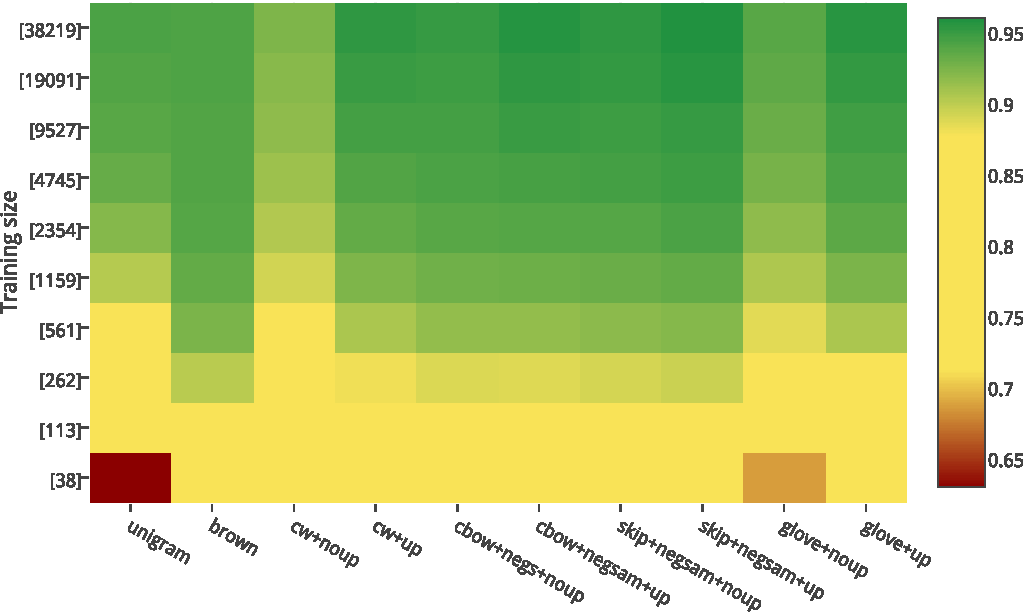
\includegraphics[scale=0.4]{plots/map-pos-color-invert.pdf}}\hfill
 \subfloat[Some other figure]{\includegraphics[width=0.48\textwidth]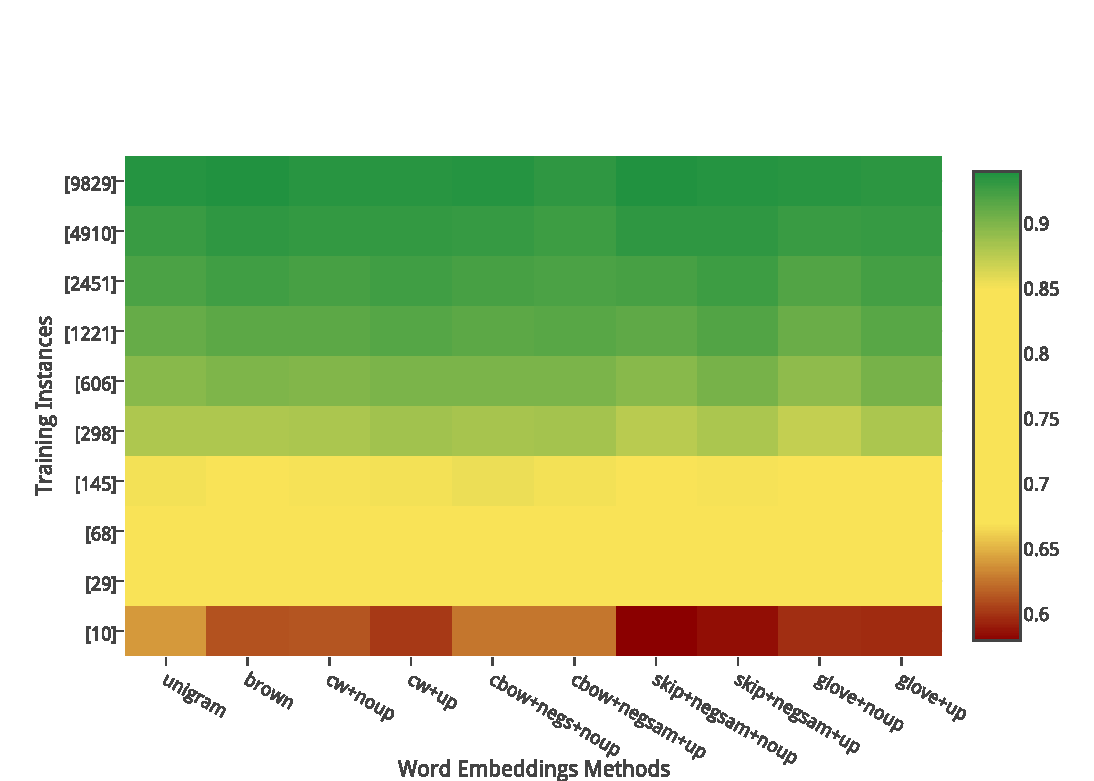
\includegraphics[scale=0.4]{plots/map-chunk-color-invert}}\\[-2ex]  %%<-- in this line
 \subfloat[Some more]{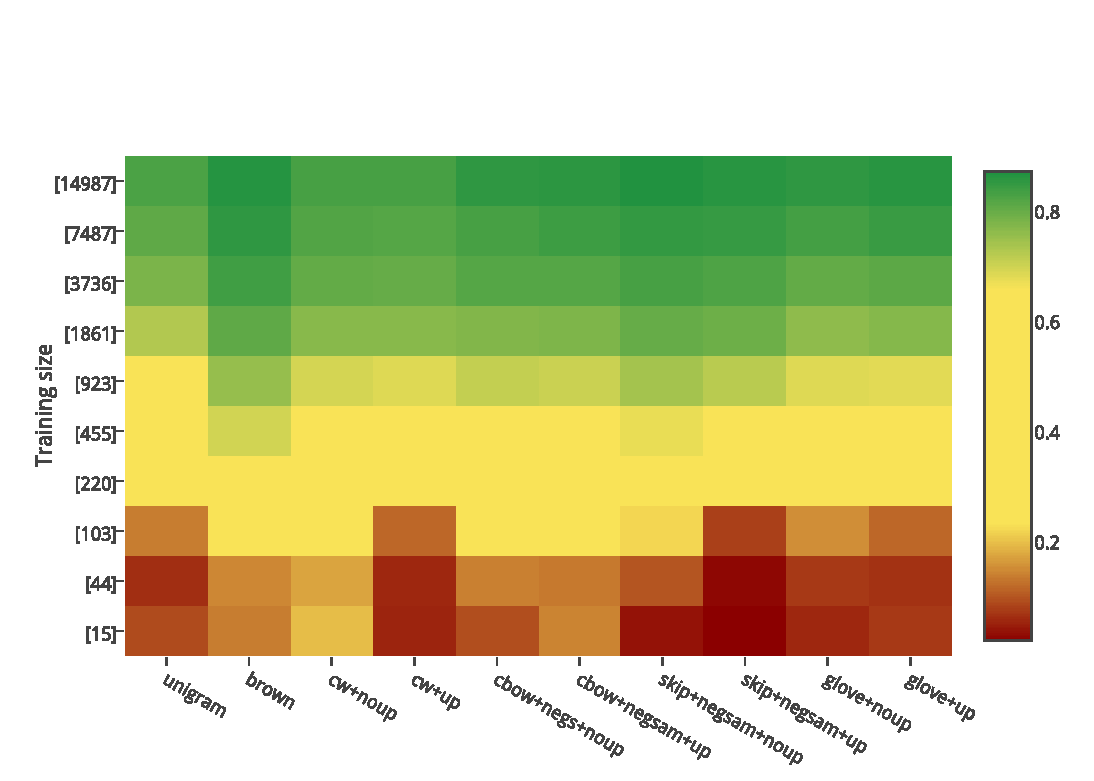
\includegraphics[scale=0.4]{plots/map-ner-color-invert}}\hfill
 \subfloat[Some less]{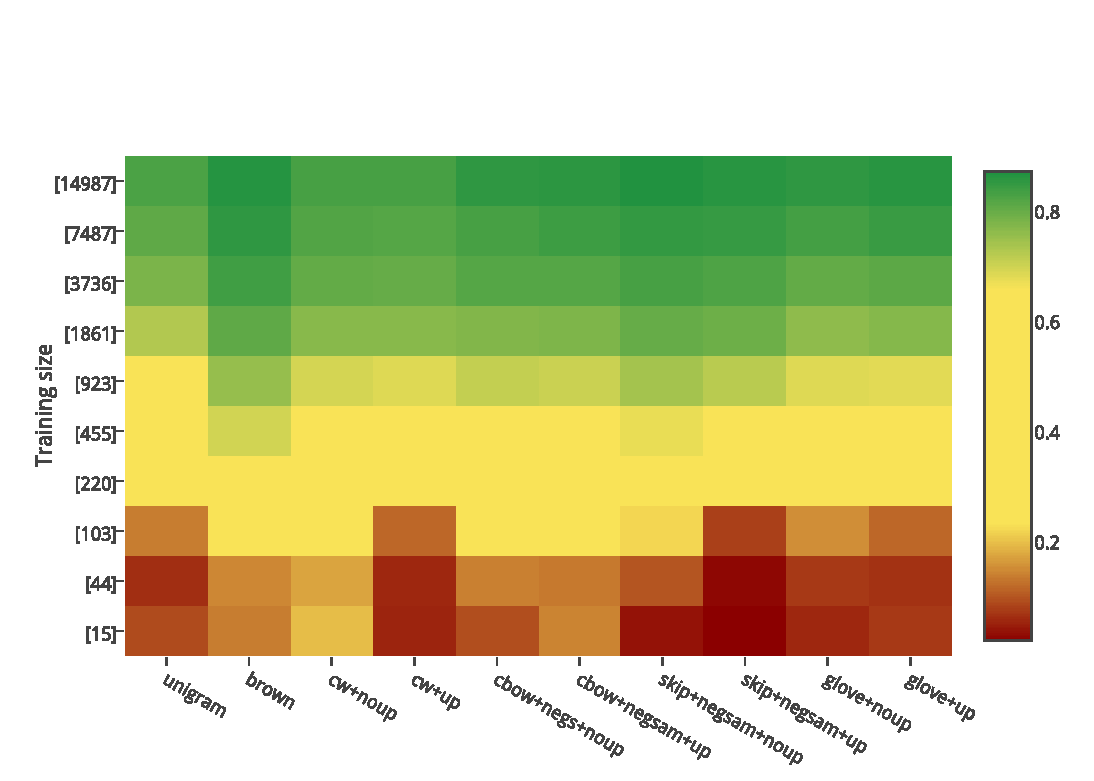
\includegraphics[scale=0.4]{plots/map-ner-color-invert}}
 \caption{There are example figures}
\end{figure}
\fi



%%%%%%%%%%%%%%%%%%%%%%%%%%%%
%%% OOV 
\begin{figure*}
\centering
\caption{Out-of-vocabulary-words (OOV) accuracy for \textit{in-domain} and \textit{out-of-domain} test sets}
\label{OOV} 
    	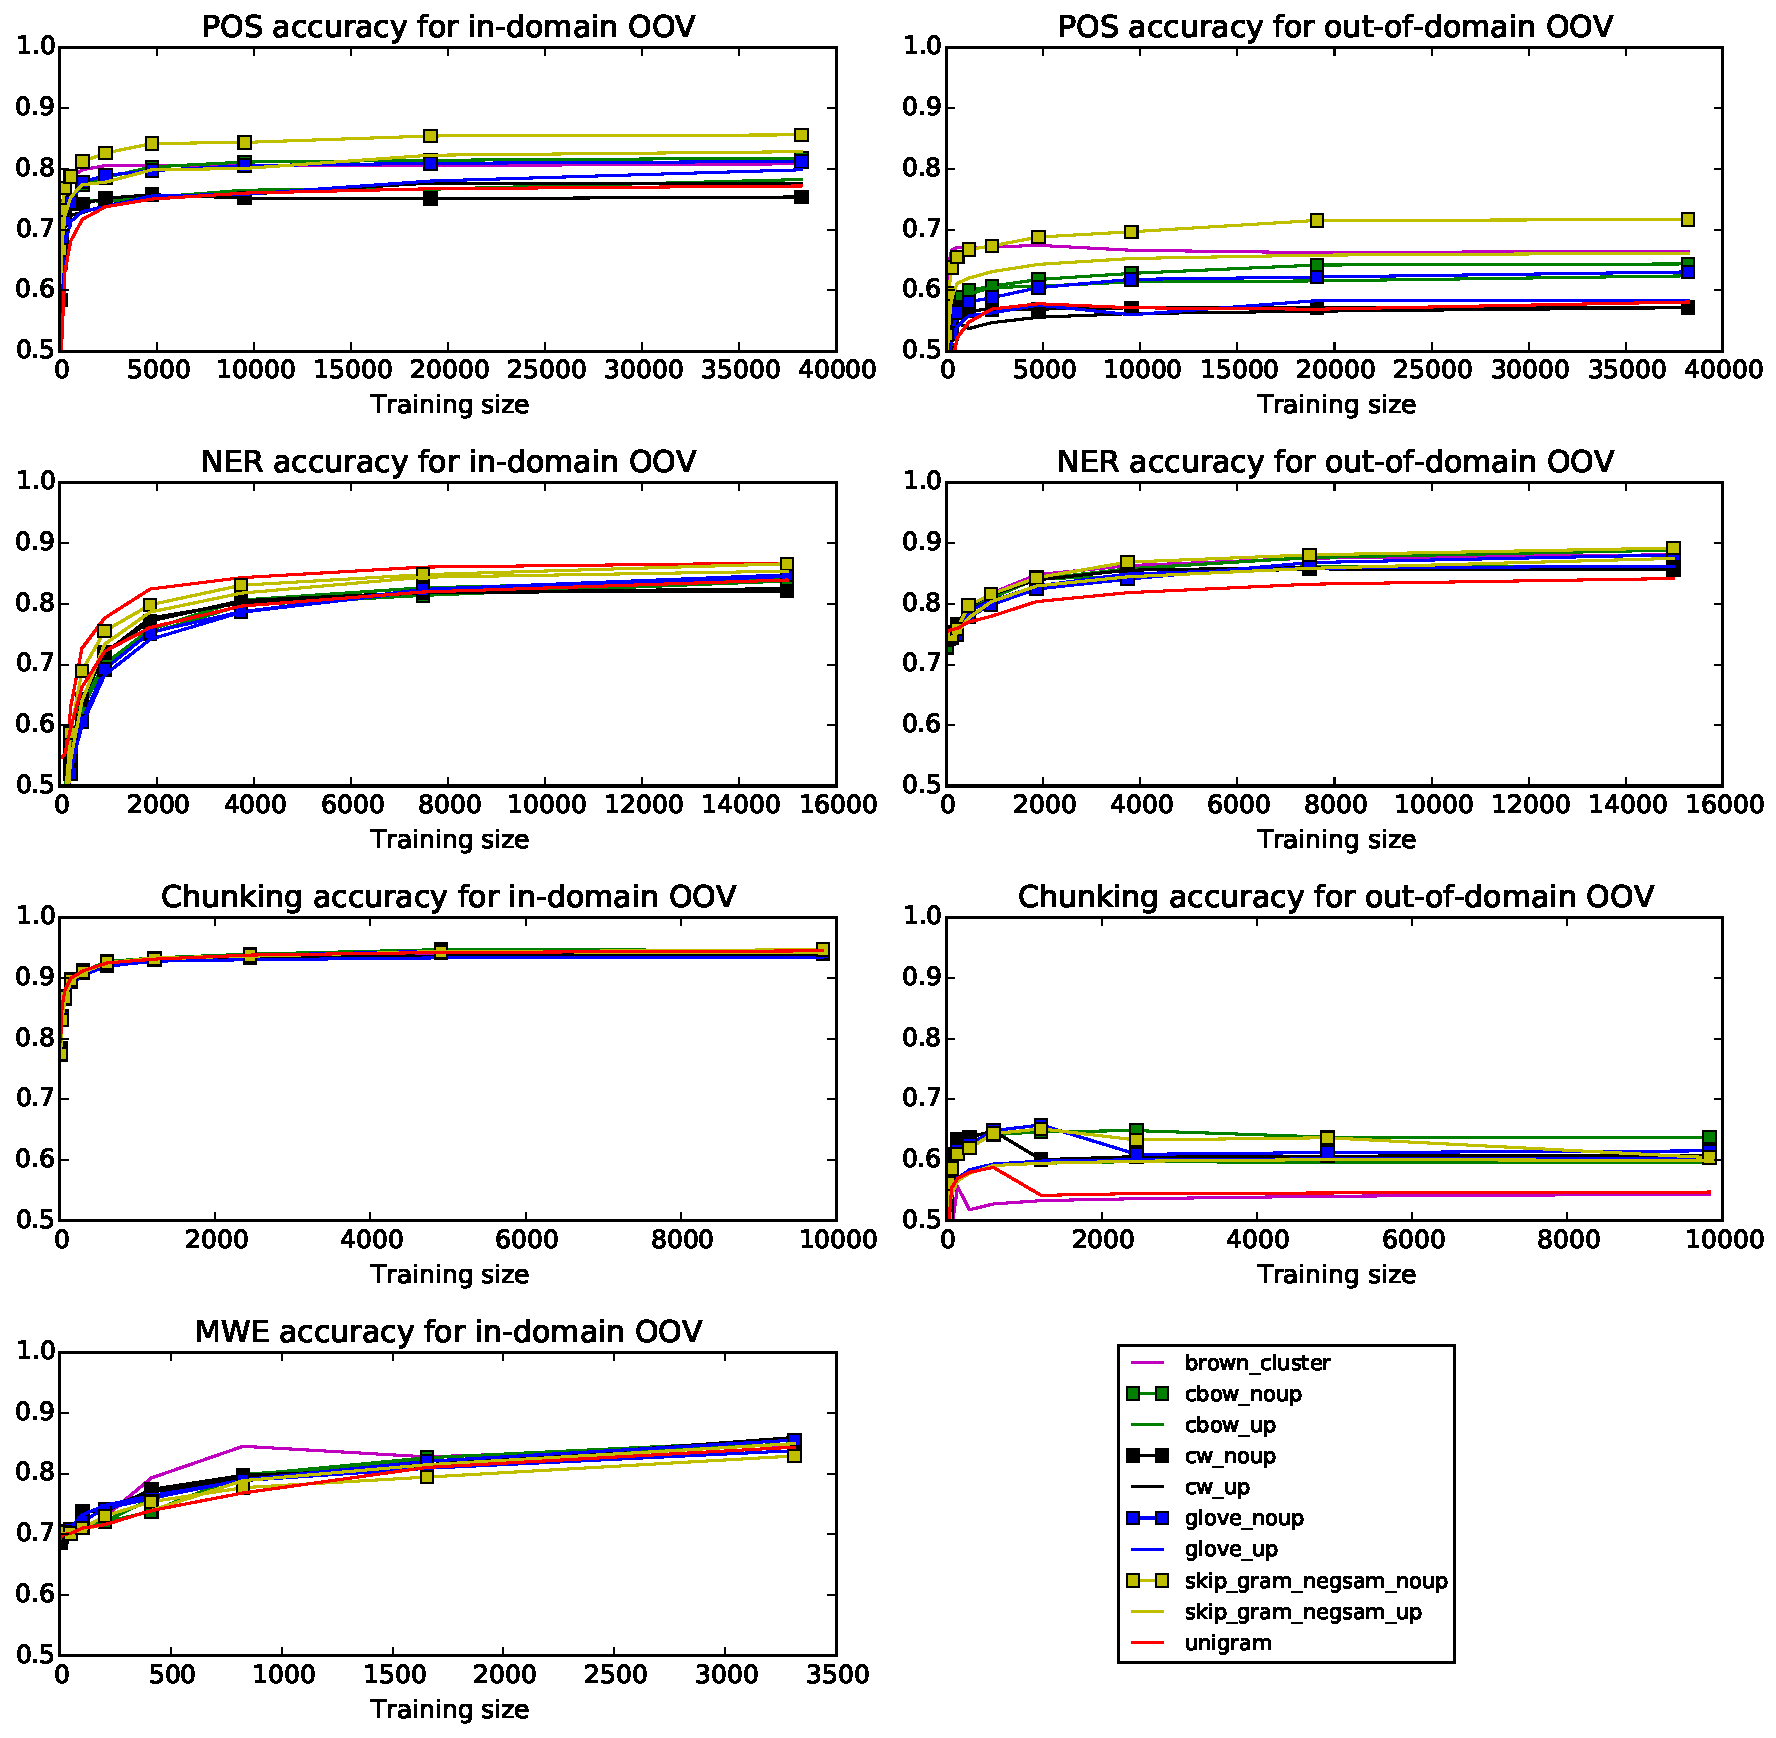
\includegraphics[scale=0.5]{plots/OOV-plots}
\end{figure*}







